\documentclass[a4paper,12pt]{report}
\usepackage[utf8]{inputenc}
\usepackage[francais]{babel}
\usepackage{graphicx}
\usepackage{fancyhdr}
\usepackage[absolute]{textpos}
\usepackage[svgnames]{xcolor}
\usepackage{colortbl}
\usepackage{lastpage}
\usepackage{url}
\usepackage[hidelinks]{hyperref}
\usepackage{geometry}
\usepackage{tikz}
\usepackage{titlesec}
\usepackage{datetime}
\usepackage{lipsum}
\usepackage{supertabular}
\usepackage{float}
\usepackage[export]{adjustbox}
\usepackage{subcaption}
\usepackage{enumerate}
\usetikzlibrary{matrix}

\newcommand{\doctitle}{AA1}
\newcommand{\doclongtitle}{Bilan architecture 1}

\title{\doctitle{} Vigilate}
\author{Soules Kévin, Mercier Daniel, Budowski Prune, Harscoat Morgane, Poncet Manuel, Keller Flavien}
\date{\today}


\definecolor{myBlue}{RGB}{23,54,93}
\definecolor{lightGray}{gray}{0.7}
\newdateformat{slashdate}{\twodigit{\THEDAY}/\twodigit{\THEMONTH}/\THEYEAR}
\newcolumntype{R}[1]{>{\centering\let\newline\\\arraybackslash\hspace{0pt}}m{#1}}

\titleformat{\section}[block]{\bfseries}{\thesection.}{1em}{}
\titleformat{\subsection}[block]{\hspace{2em}}{\thesubsection}{1em}{}
\titleformat{\subsubsection}[block]{\hspace{3em}}{\thesubsubsection}{1em}{}
  
\geometry{
  a4paper,
  left=20mm,
  right=20mm,
}

\setlength{\unitlength}{1mm}
\addtolength{\headheight}{1.5\baselineskip}
\renewcommand{\headrulewidth}{0.0pt}
\renewcommand{\footrulewidth}{0.4pt}


\fancypagestyle{eip}{
  \fancyhf{}
  \fancyhead[L] {
    \includegraphics[width=3cm]{../../logos/logo_eip.png}
  }
  \fancyhead[R] {
    \colorbox{myBlue}{
      \textcolor{white}{
        \Large \textbf{[2017][Vigilate][\doctitle{}]}
      }
    }
  }
  \renewcommand{\headrulewidth}{0pt}
  \fancyfoot[L]{
    \textcolor{gray}{
      \{EPITECH.\}
    }
  }
  \fancyfoot[C]{Vigilate}
  \fancyfoot[R]{
    \ifnum\value{page}>0
    \thepage/\pageref{LastPage}
    \fi
  }
}

\makeatletter
\let\ps@plain\ps@eip
\makeatother

\pagestyle{eip}


\begin{document}
\date{\slashdate\today}
\setcounter{page}{-3}

% --- (1) Page de garde ---

\thispagestyle{empty}
\vspace*{\stretch{2}}
\begin{center}
  \textcolor{myBlue}{\Huge \textbf{EIP Vigilate}}\linebreak
  \vspace*{\stretch{1}}
  \textcolor{gray}{\textit{\Large \doclongtitle{} (\doctitle{})}}\linebreak
  \vspace*{\stretch{1}}
  {\today}
\end{center}
\vspace*{\stretch{1}}
\newpage

% --- (2) Résumé ---

\vspace*{\stretch{1}}
\begin{flushleft}
  \textcolor{myBlue}{\textit{\large \textbf{Résumé du document}}}\linebreak
\end{flushleft}
Le cahier des charges commence par un bref rappel de notre EIP, Vigilate, un outil de sécurité informatique qui permet de se tenir informé des dernières vulnérabilités publiques rapidement sur tous les programmes que l’utilisateur souhaite vérifier. On mettra en avant les contraintes fonctionnelles et les exigences non-fonctionnelles comme le fait que notre projet doit être sécurisé, ou alors la réactivité de notre outil. Notre projet est réalisé par 6 personnes. Le document présente d’une part la structure du projet : un site web, le back-end, une machine virtuelle et un scanneur de programme et d’autre part, les différentes fonctionnalités du projet à partir d’un document UML (connexion de l’utilisateur, possibilité de modifier ses préférences : programmes à surveiller, style d’alerte souhaité...). Nous présentons dans la partie 6 l’organisation prévue : 2 personnes sur le site web, 2 sur le back-end, 1 sur la machine virtuelle et 1 sur le scanneur de programme. Ainsi que la méthodologie utilisée, basée sur la méthode Agile (Scrum). Pour ce faire, nous devons construire un produit backlog avant de commencer à développer le projet, puis organiser un nombre de sprints adéquat, d’une durée relativement courte (principe de la méthode agile) mais qui permettront d’avoir un projet fonctionnel à chaque fin de sprint avec chaque tâche décrite dans un backlog de sprint. Nous présenterons également l’environnement et les outils utilisés (github pour héberger nos documents...). Nous avons réalisé un template de mise en page pour toute notre documentation avec Latex. Nous avons choisi de respecter la norme Python Pep8 pour le développement. Dans une dernière partie, nous proposerons une description des tests, utilisés pendant le développement notamment grâce à l’outil Travis et les tests une fois l’outil terminé.\\
\vspace*{\stretch{1}}
\newpage

% --- (3) Cartouche + révisions ---

\begin{flushleft}
  \vspace*{\stretch{1}}
  \textcolor{myBlue}{\textit{\large \textbf{Description du document}}} 
  \bigbreak
  \begin{tabular}{|>{\columncolor[RGB]{220,220,220}\color{Navy}\bfseries}l|p{12cm}|}
\hline
Titre & [2017][Vigilate][\doctitle{}] \\
\hline
Date & 31/01/2015 \\
\hline
Auteur & Kévin SOULES \\
\hline
Responsable & Kévin SOULES\\
\hline
Email & vigilate\_2017@labeip.epitech.eu\\
\hline
Sujet & \doclongtitle{}\\
\hline
Mots clés & \doctitle{}, sécurité, vulnérabilités\\
\hline
Version du modèle & 1.1\\
\hline
\end{tabular}


  \vspace*{\stretch{2}}
  \bigbreak
  \bigbreak
  \textcolor{myBlue}{\textit{\large \textbf{Tableau des révisions}}}
  \bigbreak
  \small
\begin{tabular}{|p{1.5cm}|l|p{2.5cm}|p{7.8cm}|l|}
  \hline
 
   \rowcolor{Gainsboro}Date  & Auteur & Section(s) & Commentaires \\
  \hline
24/01/15 & Kévin Soules &  & Création du documents\\
  \hline
27/01/15 & Kévin Soules & Chapitre 1 et 2.1 & Recherche de liste de solutions. Rédaction du texte d'un premier concurrent. Remplissage des rappels.\\
\hline
28/01/15 & Prune Budowski & Chapitre 1 & Amélioration des rappels \\
\hline
29/01/15 & Prune Budowski & Chapitre 3.3.2 & Rédaction de la partie ``Ce qui ne sera pas couvert''\\
\hline
29/01/15 & Daniel Mercier & Chapitre 2.2 & Rédaction du texte du deuxième concurrent.\\
\hline
29/01/15 & Kévin Soules & Chapitre 2.3 & Rédaction du texte du troisième concurrent. \\
\hline
30/01/15 & Morgane Harscoat & Chapitre 2.4 & Début de rédaction du texte du quatrième concurrent. \\
\hline
30/01/15 & Kévin Soules & Chapitre 2.5 & Rédaction du texte du cinquième concurrent.\\
\hline
31/01/15 & Kévin Soules & Conclusion, Glossaire & Matrice de préférence.Rédaction d'un glossaire. \\
\hline
31/01/15 & Prune Budowski & Résumé, Conclusion, Chapitre 3.1 & Rédaction du résumé. SWOT. Rédaction de la partie ``Ce que vous apportez''.  
  \\
\hline
31/01/15 & Daniel Mercier & Toutes & Corrections. \\
31/01/15 & Prune Budowski & & Mise en page. \\
31/01/15 & Kévin Soules & & Mise en page.
\\
  \hline
\end{tabular}
\normalsize

  \vspace*{\stretch{1}}
\end{flushleft}

% --- (4) Tables des matières ---

\tableofcontents

% --- (5) Rappel eip ---

\textcolor{myBlue}{\chapter{Rappel de l'EIP}}
\setcounter{page}{1}
\section{Qu'est-ce qu’un EIP et Epitech}
Epitech,  école de l'innovation et de l'expertise informatique propose un cursus en 5 années, basé sur une pédagogie par projet (à réaliser seul ou en groupe). L'un de ces projets, l’EIP (Epitech Innovating Project), réalisé par groupes de 6 à 15 étudiants, démarre au cours de la 3\ieme année et se déroule sur 2 ans et demi. Ce  projet doit être particulièrement innovant, car son objectif est d’être commercialisable à la fin de la 5\ieme année d’Epitech.

\section{Sujet de votre EIP}
Le but de Vigilate est d’avertir les utilisateurs des services obsolètes ou potentiellement vulnérables affectant en particulier leur infrastructure (sites web, réseau d'entreprises, logiciels), dans le but de les informer des risques techniques encourus et des éventuelles mises à jour ou corrections à appliquer.
Cela sans effectuer de scan de vulnérabilité.
Nous proposons cependant un outil de scan de programme qui envoie la liste sur notre plateforme web.

\section{Glossaire}
\noindent
\vskip 0.1cm
\textbf{- C -}\\
\vskip 0.1cm
\textit{CVE (Common Vulnerabilities and Exposures)}: dictionnaire d'informations publiques relatives aux vulnérabilités informatiques. Par métonymie, on emploie souvent le terme CVE à la place de CVE ID (ou identifiant CVE), qui lui désigne le numéro qui renvoie à la fiche descriptive complète de cette vulnérabilité. Exemple: CVE-2013-4343.\\
\textit{CSIRT (Computer Security Incident Response Team)}: équipe chargée d'assurer la sécurité d'une entreprise.\\
\textit{CERT (Computer Emergency Response Team)}: marque déposée représentant les CSIRT certifiés.\\
\vskip 0.1cm
\textbf{- F -}\\
\vskip 0.1cm
\textit{Fingerprint}: déduction de la version d'un programme/système d'exploitation en fonction de la façon dont il répond à nos requêtes sur le réseau.\\
\textit{Fork}: création d'un nouveau programme en utilisant le code source du premier.\\
\vskip 0.1cm
\textbf{- G -}\\
\vskip 0.1cm
\textit{GPL (General Public License)}: licence dédiée aux logiciels libres.\\
\vskip 0.1cm
\textbf{- P -}\\
\vskip 0.1cm
\textit{Patch}: un correctif qui corrige un bug ou une vulnérabilité dans un programme.\\
\vskip 0.1cm
\textbf{- S -}\\
\vskip 0.1cm
\textit{SCADA (Supervisory Control and Data Acquisition)}: système de télégestion à grande échelle utilisé dans l'industrie.\\



\textcolor{myBlue}{\chapter{Architecture, buts et contraintes}}
\section{Contraintes fonctionnelles}
\begin{enumerate}
\item Portabilité\\
La portabilité sera la principale contrainte fonctionnelle à laquelle la réalisation du projet devra se plier.\\
  La machine virtuelle devra être conçue de façon à être utilisable sur les systèmes d'exploitation les plus répandus, il en va de même pour le site web, devant impérativement prendre en charge les 4 grands navigateurs (IE, Firefox, Google Chrome, et Safari) à jour ou non, afin que son fonctionnement ne soit pas altéré selon la configuration de l’utilisateur.\\
\item Respect des conditions légales\\
  Opérant dans le domaine de la sécurité informatique, le projet et la façon dont il sera conçu devront indubitablement se plier aux textes de loi en vigueur concernant l’informatique et les libertés relatives à ce domaine, notamment les lois imposées par la CNIL.\\
\item Analyses fréquentes
La sécurité et la stabilité faisant partie de nos exigences, et la fluidité du fonctionnement de notre système allant de paire avec, chaque ajout de code au projet devra être soumis à des vérifications et des tests unitaires, dans l'optique de conserver une structure logicielle solide et sûre.\\
Parallèlement à cela, des tentatives d'intrusions, des audits de codes, seront planifiés tous les 3 mois afin de palier aux éventuels soucis de conception pouvant mener à des risques de sécurité, qui seraient passés inaperçus lors de la mise en production.\\
\end{enumerate}
Parallèlement à cela, des tentatives d'intrusions, des audits de codes, seront planifiés tous les 3 mois afin de palier aux éventuels soucis de conception pouvant mener à des risques de sécurité, qui seraient passés inaperçus lors de la mise en production.\\

\section{Contraintes non fonctionnelles}
\begin{enumerate}
\item Simplicité de l'interface\\
 Dans un souci de simplicité d'utilisation, il faudra que l'interface utilisateur de notre système soit intuitive et à la portée de tous, de façon à favoriser la prise en main de cette solution par un utilisateur lambda, n'ayant aucune compétence avancée en informatique.\\
 Différents types d'alertes pourront être envoyés au client, une alerte détaillée concernant la vulnérabilité, ses détails techniques et ses caractéristiques, pouvant être destinée à l'équipe informatique du client, et une alerte plus concise pouvant par exemple être destinée à un responsable.\\
\item Réactivité
  Afin d'optimiser l'efficacité de notre solution, la réactivité est l'un des points clés à respecter.\\
  Dans le but d'informer les utilisateurs des vulnérabilités les concernant dans les plus brefs délais, nous nous devrons de concevoir et maintenir un système réactif au niveau la récupération et la transmission des données, devant mettre moins de 5 secondes à avertir un utilisateur concerné par une faille via les notifications sur notre site, et moins d’une minute par mail et sms.\\
  Cela permettant au client de faire corriger les vulnérabilités de son système au plus vite.\\
\item Concevoir un système et une plateforme sécurisés\\
  Le but de notre solution étant de favoriser la sûreté des services utilisés par nos clients, avoir un produit et une infrastructure stable fait également partie des points clés à respecter.\\
  Il sera donc impératif de sécuriser correctement le site, les différents services que nous utilisons et par conséquent, nos données via chiffrement des données utilisateurs et des espaces de stockages, afin d'éviter toutes fuites de données relatives à un client, à son système informatique, ou à notre propre infrastructure.\\ 
\end{enumerate}
Enfin, le système en machine virtuelle destiné à être installé chez le client devra être développé de façon à être imperméable à toute forme d'attaque actuellement prévisible, il va de soi qu'après sa fonction principale de détection et d'alerte, la priorité de ce système concerne le fait qu'il ne puisse, ou le moins possible, être lui-même compromis par une attaque informatique.\\
Des tests de sécurité seront effectués tous les 3 mois sur la plateforme ainsi que la machine virtuelle.\\


\textcolor{myBlue}{\chapter{Vue globale du projet}}
\section{Use Cases principaux }

\begin{figure}[H]
  \caption{Diagramme UML use case}
  \centering
  \vspace*{0.5cm}
  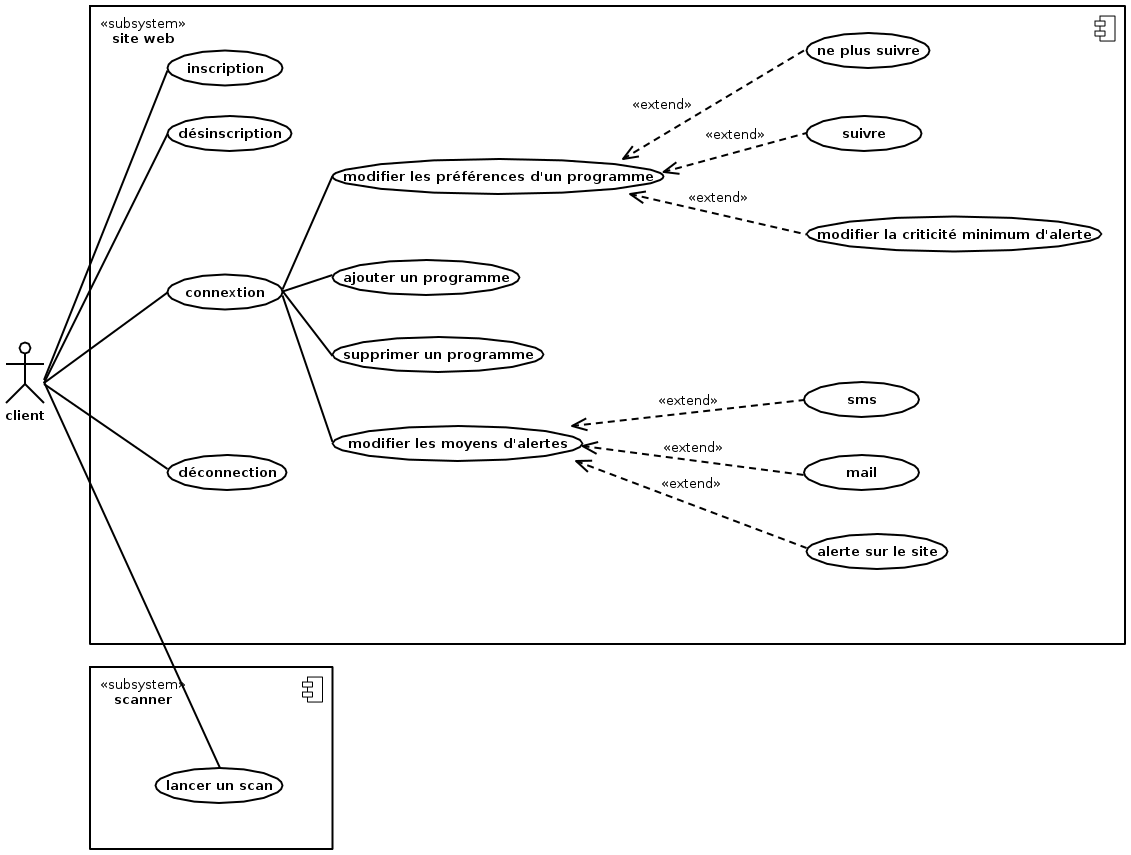
\includegraphics[width=10cm]{usecase.png}
\end{figure}

\section{Use cases détaillés}
Le client peut : s'inscrire, se désinscire, se connecter, se déconnecter, lancer le programme de scan sur sa machine.\\
Dans le cas de la connexion, l'utilisateur peut:\\
\begin{itemize}
\item Modifier les préférences d'un programme (suivre/ne plus suivre/modifier la criticité)\\
\item Ajouter un programme\\
\item Supprmer un programme\\
\item Modifier les moyens d'alertes (sms/mail/alerte sur le site\\
\end{itemize}

\textcolor{myBlue}{\chapter{Vue Logique de l’application}}
\section{Vue globale}
Voici un diagramme qui représente les différents composants de vigilate.
\begin{figure}[H]
  \caption{Diagramme de composants}
  \centering
  \vspace*{0.5cm}
  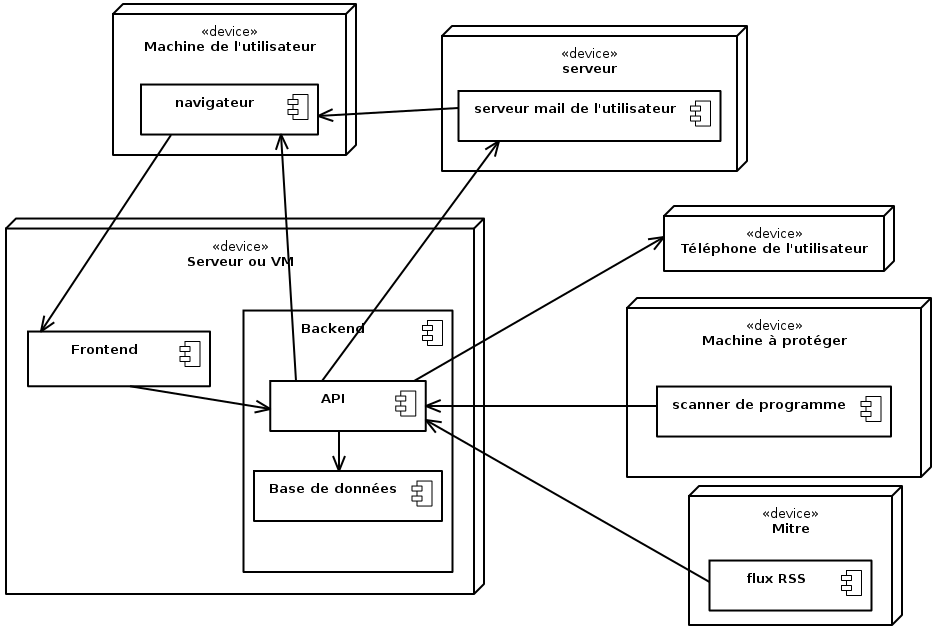
\includegraphics[width=15cm]{composants.png}
\end{figure}
\section{Composants principaux}

Un certain nombre de composants présent dans le diagramme ci-dessus existe déjà : le navigateur, le téléphone, le serveur mail et le flux RSS de mitre. Nous allons donc utiliser ces composants dans l’état dans lequel ils existent aujourd’hui.\\
Le navigateur servira à accéder au frontend pour paramétrer la solution ainsi qu’as recevoir les alertes levés par le backend (directement sur le navigateur ou via un email envoyé lui aussi par le backend).
Le serveur de mail servira juste à recevoir les emails d’alerte envoyé par le backend.\\
Le téléphone ne servira lui aussi qu’as recevoir les alertes, cette fois via un SMS.\\
Le flux RSS de mitre sert à recevoir les informations des nouvelles vulnérabilités découvertes.\\
Pour ce qui est des composants restants, à savoir le frontend, le backand (api et base de données) ainsi que le scanner de programmes, nous allons devoir les développer.\\
Le frontend serviras d’interface pour l’utilisateur afin de pouvoir paramétrer la solution Vigilate.\\
Le backend auras pour rôle de récupérer les informations sur les nouvelles vulnérabilités et la liste des programme installé ainsi que de lever des alertes de sécurité lorsqu’un utilisateur est vulnérable. Le backend utilise les paramètre entré par l’utilisateur pour savoir si une alerte doit être levé et par quel moyen.\\
Le scanner de programme sert à faciliter l’utilisation de Vigilate, en effet, il permet à l’utilisateur de mettre à jour automatiquement la liste des programmes installer sans avoir à les ajouter tous à la main via le frontend.\\


\textcolor{myBlue}{\chapter{Implémentation}}
\section{Vue globale}

\begin{figure}[H]
  \caption{Architecture trois tiers}
  \centering
  \vspace*{0.5cm}
  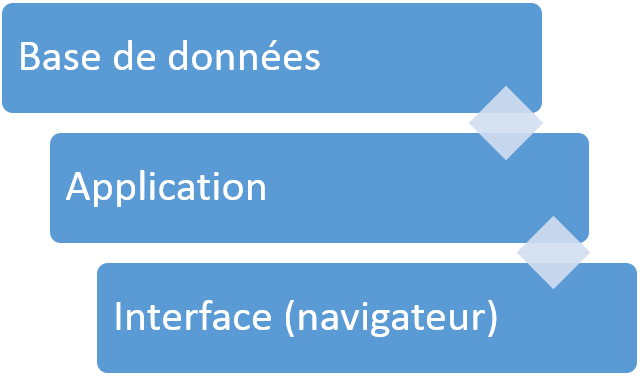
\includegraphics[width=10cm]{implem_1.png}
\end{figure}
Couche de présentation – Premier niveau : Interface web par navigateur.\\
Il s’agit d’une interface web qui permet au client d’interagir avec la solution.\\
Cette couche a pour vocation de relayer les requêtes de l’utilisateur à destination de la couche métier mais aussi d’afficher les informations envoyées par la couche métier à celle-ci. On parle donc d’une interface homme machine.\\
La couche de présentation sera disponible au travers d’une interface web utilisant le framework Django, adoptant un modèle MVT (Modèle-Vue-Template) :\\
\begin{figure}[H]
  \caption{Modèle MVT}
  \centering
  \vspace*{0.5cm}
  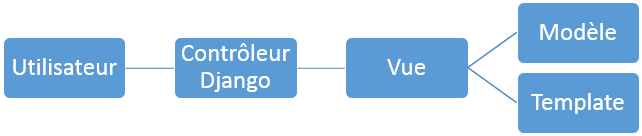
\includegraphics[width=15cm]{implem_2.png}
\end{figure}
\noindent
Couche métier – Second niveau : Application et interpréteur de données.\\
L’application aura pour vocation d’interpréter les données envoyées par la couche d’accès aux données, de les rendre intelligibles, et de les transmettre à la couche de présentation.\\
Elle permettra aussi de communiquer les requêtes de la couche présentation à la couche d’accès aux données en effectuant le travail inverse, transformer une requête simple émise par le premier niveau en langage complexe compréhensible par le troisième niveau. En résumé, la couche métier a pour objectif le traitement des données qui transitent entre le premier niveau et le troisième niveau et de s’assurer que les données soient compréhensibles pour les niveaux en les transformant au format adéquat.\\
Couche d’accès aux données – Troisième niveau : Basse de donnée et corrélation
Cette couche a pour but de stocker des données et de les rendre facilement accessibles pour la couche métier.  Les données stockées seront sauvegardées et/ou archivées parce qu’elles sont destinées à rester de manière définitive dans la base. Cette couche est aussi capable de recevoir des ordres interprétés par la couche métier.\\
\section{Couches applicatives}

\begin{figure}[H]
  \caption{Couche applicative}
  \centering
  \vspace*{0.5cm}
  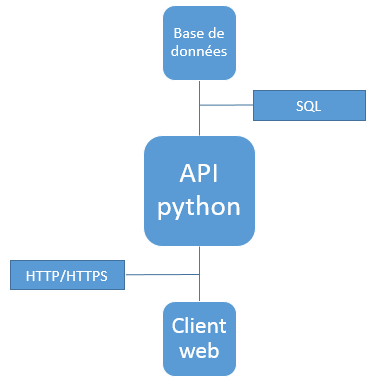
\includegraphics[width=10cm]{implem_3.png}
\end{figure}


\textcolor{myBlue}{\chapter{Taille et Performance}}
La vitesse de transmission des information étant un point clé de ce projet, les délais d’envois des notifications aux clients seront les plus courts possible, avec un objectif de moins d’une minute pour l’envoi d’email et de sms, et 5 secondes pour une notification sur le site web.\\
Le système de base de données devra lui, disposer d’un espace de stockage de plusieurs teraoctets permettant de stocker en premier lieu les informations relatives à un maximum de vulnérabilités passées actuelles et futures, ainsi que les données de chaque client. L’état actuel du projet ne nous permet pas de donner une estimation plus précise de l’espace de stockage nécessaire.\\


\textcolor{myBlue}{\chapter{Qualité}}
Nous avons pensé à un site web pour Vigilate pour une utilisation plus simplifié pour l'utilisateur qu'un logiciel bureau. En effet il n'y a pas besoin d'installation. il suffit d'un mot de passe pour se connecter et donc l'utilisateur peut se connecter et faire marcher Vigilate depuis n'importe quelle machine.
Pour l'extensibilité de notre projet, l'utilisateur n'aura rien à faire non plus comme c'est un site web les mises à jour pourront passer inaperçues et donc ne pas compliquer l'utilisation. 

\end{document}